\chapter{Background}

This chapter provides an overview of the related topics for this master thesis.

\section{TG799-vac}

The OpenWrt-based router examined in this thesis, see Figure \ref{fig:tg799}, is commonly known as TG799, manufactured by Technicolor with Broadcom and Quantenna modems. A custom firmware was used to gain root access over SSH.

\begin{figure}
\center
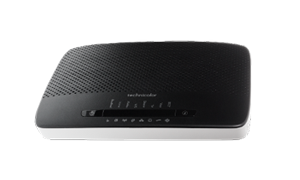
\includegraphics[width=0.5\textwidth]{images/tg799.png}
\caption{The TG799 router from Technicolor}
\label{fig:tg799}
\end{figure}

\section{IEEE 802.11}

The ubiquitous set of LAN standards for wireless communication. Specify MAC and PHY protocols.

Basic protocol description, relevant for this master thesis.

How later standards IEEE 802.11b g n ac change.

\section{ubus - the OpenWrt micro bus architecture}

A client program which acts as an interface to the bus daemon, \texttt{ubusd}. Input and output format is JSON.

The router registers a namespace called \texttt{wireless} and this is what we call to find the meaning of life.

\section{Deutche telekom supra}

Björns oklara vapen.

\section{Rhode \& Schwarz FWLZ-XYZ}

(not broken) network analyser;

\section{Wi-Spy Channalyzer}

the wi-spy, top secret agent auf d00m.
